\documentclass[crop, tikz]{standalone}
\usepackage{tikz}
\usepackage[english]{babel}
\usepackage[utf8]{inputenc}
\usepackage{anyfontsize}
\usetikzlibrary{calc}
\usetikzlibrary{positioning,arrows.meta,shadows}
\usetikzlibrary{arrows,shapes, decorations.pathmorphing,backgrounds,positioning, shapes.geometric,fit}


\begin{document}
    \begin{tikzpicture}[square/.style={regular polygon,regular polygon sides=4}]
        %% Graph 1 (V,E)
     	\node[circle, thick, draw] (0) {$\vec{x}_i$};
        \node[circle, thick, draw, above right=0.1em and 3em of 0] (1) {};
        \node[circle, thick, draw, above right=0.8em and 0.5em of 0] (2) {};
        \node[circle, thick, draw, left=of 0] (3) {};
        \node[circle, thick, draw, below left=0.8em and 1.5em of 0] (4) {};
        
        \draw[-, thick] (0) -- (1);
        \draw[-, thick] (0) -- (2);
        \draw[-, thick] (0) -- (3);
        \draw[-, thick] (4) -- (3);
        
        \node[rectangle, draw, dashed, minimum width=11em, minimum height=5.5em] (RR) {};
        \node[below=0em of RR] (l1) {$({\bf V}, {\bf E})$};

        \begin{lrbox}{0}
        \begin{scope}
            %% Message passing
            \draw[->, line width=0.5mm, color=cyan!70!black] (1) -- (0);
            \draw[->, line width=0.5mm, color=cyan!70!black] (2) -- (0);
            \draw[->, line width=0.5mm, color=cyan!70!black] (3) -- (0);
            
            \path[draw,line width=5pt,-,cyan!70!black, opacity=0.4] (1) -- (0);
            \path[draw,line width=5pt,-,cyan!70!black, opacity=0.4] (2) -- (0);
            \path[draw,line width=5pt,-,cyan!70!black, opacity=0.4] (3) -- (0);
            
            \node[circle, ultra thick, draw, draw=cyan!70!black, text opacity=0] (m1) at ($(0)$) {$\vec{x}_i$};
    
    
            %% Graph 2 (H,E)
            \node[rectangle, draw, dashed, minimum width=11em, minimum height=5.5em, right=12.5em of 0] (AA) {};
            \node[below=0em of AA] (l1) {\begin{tabular}{c}
                 Latents \\
                 $({\bf H}, {\bf E})$
            \end{tabular}};
            
            \node[circle, ultra thick, draw, right=17em of 0, fill=cyan!70!black, draw=cyan!70!black,fill opacity=.2,text opacity=1] (0) {$\vec{h}_i$};
            \node[circle, thick, draw, above right=0.1em and 3em of 0] (1) {};
            \node[circle, thick, draw, above right= 0.8em and 0.5em of 0] (2) {};
            \node[circle, thick, draw, left=of 0] (3) {};
            \node[circle, thick, draw, below left=0.8em and 1.5em of 0] (4) {};
            
            \draw[-, thick] (0) -- (1);
            \draw[-, thick] (0) -- (2);
            \draw[-, thick] (0) -- (3);
            \draw[-, thick] (4) -- (3);
            
            %%%%%%%%%%%%%%%%%%%%%%%%%
            %% GNN connector
            \draw[-stealth, very thick, decoration={snake, pre length=0.01mm, segment length=2mm, amplitude=0.3mm, post length=1.5mm}, decorate,color=cyan!70!black] (RR) -- node[above] {GNN} (AA);
            %%%%%%%%%%%%%%%%%%%%%%%%%

            %% Node classification
            \node[square, ultra thick, draw, above right=of AA, fill=magenta, draw=magenta!80!black,fill opacity=.2,text opacity=1, draw opacity=1] (ZJ) {$\vec{z}_i$};
            \draw[-stealth, very thick, decoration={snake, pre length=0.01mm, segment length=2mm, amplitude=0.3mm, post length=1.5mm}, decorate,color=magenta!80!black] (0) to[out=90,in=180] (ZJ);
            \node[right=0em of ZJ] (zj1) {\begin{tabular}{l}
                 \textcolor{magenta!80!black}{Node} classification \\
                 $\vec{z}_i = f(\vec{h}_i)$
            \end{tabular}};
            \node[square, ultra thick, draw, right=of AA, fill=green, draw=green!70!black,fill opacity=.2,text opacity=1] (ZG) {$\vec{z}_G$};
            \node[right=0em of ZG] (zj1) {\begin{tabular}{l}
                 \textcolor{green!70!black}{Graph} classification \\
                 $\vec{z}_G = f(\sum_i \vec{h}_i)$
            \end{tabular}};
            \draw[-stealth, very thick, decoration={snake, pre length=0.01mm, segment length=2mm, amplitude=0.3mm, post length=1.5mm}, decorate,color=green!70!black] (0) to[out=350,in=180] (ZG);
            \draw[-stealth, very thick, decoration={snake, pre length=0.01mm, segment length=2mm, amplitude=0.3mm, post length=1.5mm}, decorate,color=green!70!black] (1) to[out=350,in=170] (ZG);
            \draw[-stealth, very thick, decoration={snake, pre length=0.01mm, segment length=2mm, amplitude=0.3mm, post length=1.5mm}, decorate,color=green!70!black] (2) to[out=45,in=160] (ZG);
            \draw[-stealth, very thick, decoration={snake, pre length=0.01mm, segment length=2mm, amplitude=0.3mm, post length=1.5mm}, decorate,color=green!70!black] (3) to[out=320,in=190] (ZG);
            \draw[-stealth, very thick, decoration={snake, pre length=0.01mm, segment length=2mm, amplitude=0.3mm, post length=1.5mm}, decorate,color=green!70!black] (4) to[out=350,in=200] (ZG);
            \node[square, ultra thick, draw, below right=of AA, fill=blue, draw=blue,fill opacity=.2,text opacity=1] (ZIJ) {$\vec{z}_{ij}$};
            \node[right=0em of ZIJ] (zj1) {\begin{tabular}{l}
                 \textcolor{blue}{Edge} classification \\
                 $\vec{z}_{ij} = f(\vec{h}_i,\vec{h}_j,\vec{e}_{ij})$
            \end{tabular}};
            \draw[-stealth, very thick, decoration={snake, pre length=0.01mm, segment length=2mm, amplitude=0.3mm, post length=1.5mm}, decorate,color=blue] (0) to[out=320,in=180] (ZIJ);
            \draw[-stealth, very thick, decoration={snake, pre length=0.01mm, segment length=2mm, amplitude=0.3mm, post length=1.5mm}, decorate,color=blue] (1) to[out=270,in=160] (ZIJ);

            %%%%
            \node[circle, ultra thick, draw, draw=blue, text opacity=0] (m1) at ($(0)$) {$\vec{h}_i$};
            	    
            \node[circle, ultra thick, draw, draw=blue, text opacity=0] (m1) at ($(1)$) {};
            	    
            \draw[<->, line width=0.5mm, color=blue] (1) -- (0);
            \path[draw,line width=5pt,-,blue, opacity=0.4] (1) -- (0);
        \end{scope}
        \end{lrbox}
    \end{tikzpicture}
        
        %%%%%%%%%%%%%%%%%%%%%%%%%
    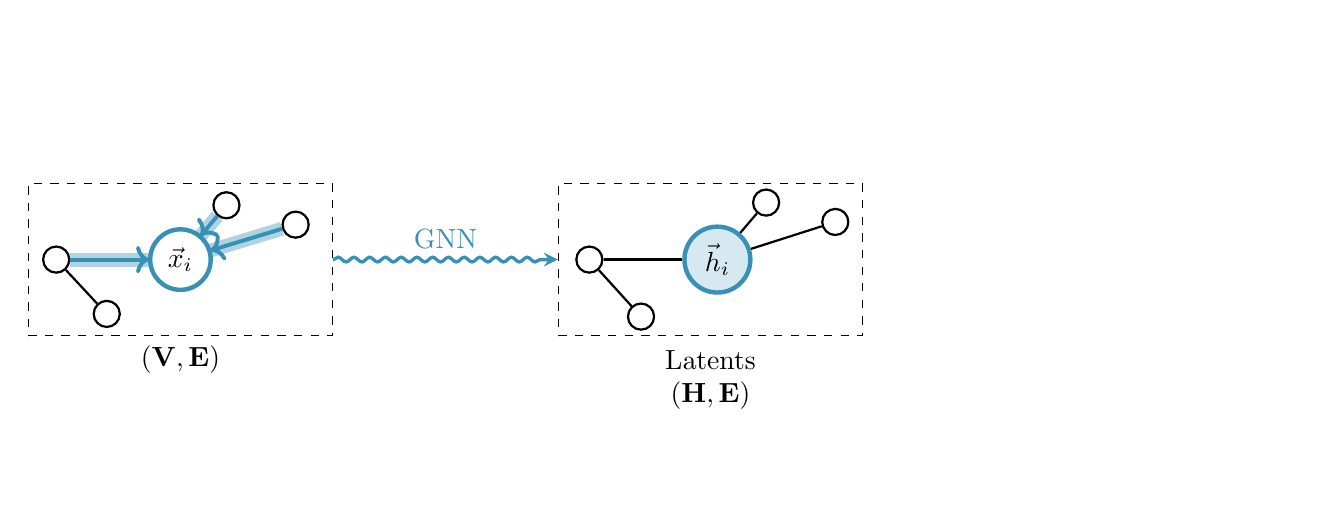
\begin{tikzpicture}[square/.style={regular polygon,regular polygon sides=4}]
        %% Graph 1 (V,E)
     	\node[circle, thick, draw] (0) {$\vec{x}_i$};
        \node[circle, thick, draw, above right=0.1em and 3em of 0] (1) {};
        \node[circle, thick, draw, above right=0.8em and 0.5em of 0] (2) {};
        \node[circle, thick, draw, left=of 0] (3) {};
        \node[circle, thick, draw, below left=0.8em and 1.5em of 0] (4) {};
        
        \draw[-, thick] (0) -- (1);
        \draw[-, thick] (0) -- (2);
        \draw[-, thick] (0) -- (3);
        \draw[-, thick] (4) -- (3);
        
        \node[rectangle, draw, dashed, minimum width=11em, minimum height=5.5em] (RR) {};
        \node[below=0em of RR] (l1) {$({\bf V}, {\bf E})$};

        %% Message passing
        \draw[->, line width=0.5mm, color=cyan!70!black] (1) -- (0);
        \draw[->, line width=0.5mm, color=cyan!70!black] (2) -- (0);
        \draw[->, line width=0.5mm, color=cyan!70!black] (3) -- (0);
        
        \path[draw,line width=5pt,-,cyan!70!black, opacity=0.4] (1) -- (0);
        \path[draw,line width=5pt,-,cyan!70!black, opacity=0.4] (2) -- (0);
        \path[draw,line width=5pt,-,cyan!70!black, opacity=0.4] (3) -- (0);
        
        \node[circle, ultra thick, draw, draw=cyan!70!black, text opacity=0] (m1) at ($(0)$) {$\vec{x}_i$};
    
    
        %% Graph 2 (H,E)
        \node[rectangle, draw, dashed, minimum width=11em, minimum height=5.5em, right=12.5em of 0] (AA) {};
        \node[below=0em of AA] (l1) {\begin{tabular}{c}
             Latents \\
             $({\bf H}, {\bf E})$
        \end{tabular}};
        
        \node[circle, ultra thick, draw, right=17em of 0, fill=cyan!70!black, draw=cyan!70!black,fill opacity=.2,text opacity=1] (0) {$\vec{h}_i$};
        \node[circle, thick, draw, above right=0.1em and 3em of 0] (1) {};
        \node[circle, thick, draw, above right= 0.8em and 0.5em of 0] (2) {};
        \node[circle, thick, draw, left=of 0] (3) {};
        \node[circle, thick, draw, below left=0.8em and 1.5em of 0] (4) {};
        
        \draw[-, thick] (0) -- (1);
        \draw[-, thick] (0) -- (2);
        \draw[-, thick] (0) -- (3);
        \draw[-, thick] (4) -- (3);
        
        %%%%%%%%%%%%%%%%%%%%%%%%%
        %% GNN connector
        \draw[-stealth, very thick, decoration={snake, pre length=0.01mm, segment length=2mm, amplitude=0.3mm, post length=1.5mm}, decorate,color=cyan!70!black] (RR) -- node[above] {GNN} (AA);
        %%%%%%%%%%%%%%%%%%%%%%%%%

        \begin{lrbox}{0}
        \begin{scope}
            %% Node classification
            \node[square, ultra thick, draw, above right=of AA, fill=magenta, draw=magenta!80!black,fill opacity=.2,text opacity=1, draw opacity=1] (ZJ) {$\vec{z}_i$};
            \draw[-stealth, very thick, decoration={snake, pre length=0.01mm, segment length=2mm, amplitude=0.3mm, post length=1.5mm}, decorate,color=magenta!80!black] (0) to[out=90,in=180] (ZJ);
            \node[right=0em of ZJ] (zj1) {\begin{tabular}{l}
                 \textcolor{magenta!80!black}{Node} classification \\
                 $\vec{z}_i = f(\vec{h}_i)$
            \end{tabular}};
            \node[square, ultra thick, draw, right=of AA, fill=green, draw=green!70!black,fill opacity=.2,text opacity=1] (ZG) {$\vec{z}_G$};
            \node[right=0em of ZG] (zj1) {\begin{tabular}{l}
                 \textcolor{green!70!black}{Graph} classification \\
                 $\vec{z}_G = f(\sum_i \vec{h}_i)$
            \end{tabular}};
            \draw[-stealth, very thick, decoration={snake, pre length=0.01mm, segment length=2mm, amplitude=0.3mm, post length=1.5mm}, decorate,color=green!70!black] (0) to[out=350,in=180] (ZG);
            \draw[-stealth, very thick, decoration={snake, pre length=0.01mm, segment length=2mm, amplitude=0.3mm, post length=1.5mm}, decorate,color=green!70!black] (1) to[out=350,in=170] (ZG);
            \draw[-stealth, very thick, decoration={snake, pre length=0.01mm, segment length=2mm, amplitude=0.3mm, post length=1.5mm}, decorate,color=green!70!black] (2) to[out=45,in=160] (ZG);
            \draw[-stealth, very thick, decoration={snake, pre length=0.01mm, segment length=2mm, amplitude=0.3mm, post length=1.5mm}, decorate,color=green!70!black] (3) to[out=320,in=190] (ZG);
            \draw[-stealth, very thick, decoration={snake, pre length=0.01mm, segment length=2mm, amplitude=0.3mm, post length=1.5mm}, decorate,color=green!70!black] (4) to[out=350,in=200] (ZG);
            \node[square, ultra thick, draw, below right=of AA, fill=blue, draw=blue,fill opacity=.2,text opacity=1] (ZIJ) {$\vec{z}_{ij}$};
            \node[right=0em of ZIJ] (zj1) {\begin{tabular}{l}
                 \textcolor{blue}{Edge} classification \\
                 $\vec{z}_{ij} = f(\vec{h}_i,\vec{h}_j,\vec{e}_{ij})$
            \end{tabular}};
            \draw[-stealth, very thick, decoration={snake, pre length=0.01mm, segment length=2mm, amplitude=0.3mm, post length=1.5mm}, decorate,color=blue] (0) to[out=320,in=180] (ZIJ);
            \draw[-stealth, very thick, decoration={snake, pre length=0.01mm, segment length=2mm, amplitude=0.3mm, post length=1.5mm}, decorate,color=blue] (1) to[out=270,in=160] (ZIJ);

            %%%%
            \node[circle, ultra thick, draw, draw=blue, text opacity=0] (m1) at ($(0)$) {$\vec{h}_i$};
            	    
            \node[circle, ultra thick, draw, draw=blue, text opacity=0] (m1) at ($(1)$) {};
            	    
            \draw[<->, line width=0.5mm, color=blue] (1) -- (0);
            \path[draw,line width=5pt,-,blue, opacity=0.4] (1) -- (0);
        \end{scope}
        \end{lrbox}
    \end{tikzpicture}
    
    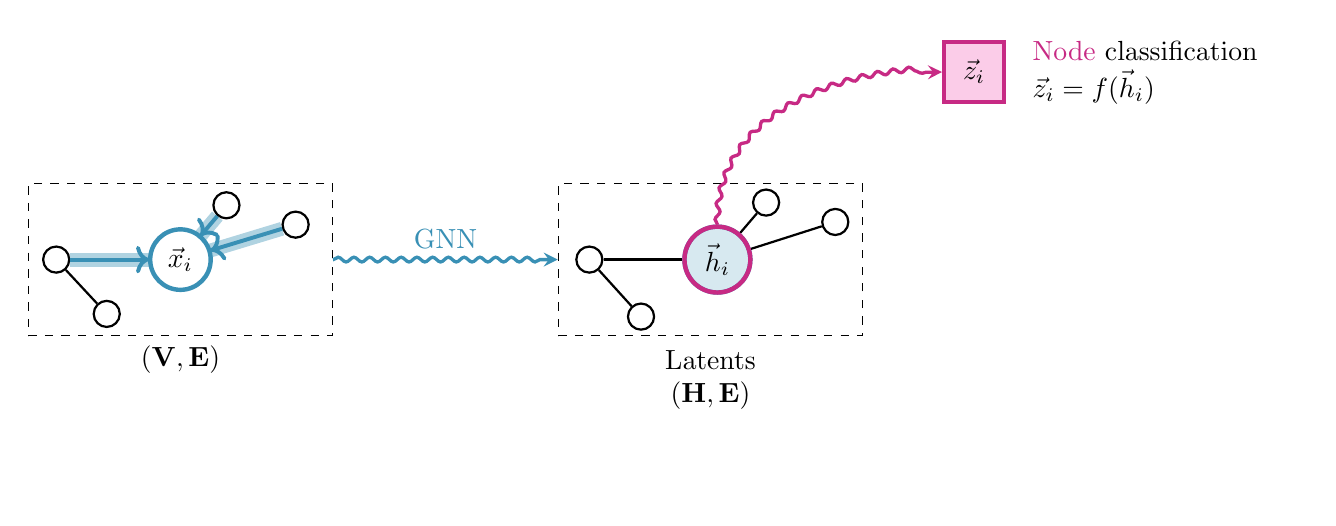
\begin{tikzpicture}[square/.style={regular polygon,regular polygon sides=4}]
        %% Graph 1 (V,E)
     	\node[circle, thick, draw] (0) {$\vec{x}_i$};
        \node[circle, thick, draw, above right=0.1em and 3em of 0] (1) {};
        \node[circle, thick, draw, above right=0.8em and 0.5em of 0] (2) {};
        \node[circle, thick, draw, left=of 0] (3) {};
        \node[circle, thick, draw, below left=0.8em and 1.5em of 0] (4) {};
        
        \draw[-, thick] (0) -- (1);
        \draw[-, thick] (0) -- (2);
        \draw[-, thick] (0) -- (3);
        \draw[-, thick] (4) -- (3);
        
        \node[rectangle, draw, dashed, minimum width=11em, minimum height=5.5em] (RR) {};
        \node[below=0em of RR] (l1) {$({\bf V}, {\bf E})$};

        %% Message passing
        \draw[->, line width=0.5mm, color=cyan!70!black] (1) -- (0);
        \draw[->, line width=0.5mm, color=cyan!70!black] (2) -- (0);
        \draw[->, line width=0.5mm, color=cyan!70!black] (3) -- (0);
        
        \path[draw,line width=5pt,-,cyan!70!black, opacity=0.4] (1) -- (0);
        \path[draw,line width=5pt,-,cyan!70!black, opacity=0.4] (2) -- (0);
        \path[draw,line width=5pt,-,cyan!70!black, opacity=0.4] (3) -- (0);
        
        \node[circle, ultra thick, draw, draw=cyan!70!black, text opacity=0] (m1) at ($(0)$) {$\vec{x}_i$};
    
    
        %% Graph 2 (H,E)
        \node[rectangle, draw, dashed, minimum width=11em, minimum height=5.5em, right=12.5em of 0] (AA) {};
        \node[below=0em of AA] (l1) {\begin{tabular}{c}
             Latents \\
             $({\bf H}, {\bf E})$
        \end{tabular}};
        
        \node[circle, ultra thick, draw, right=17em of 0, fill=cyan!70!black, draw=cyan!70!black,fill opacity=.2,text opacity=1] (0) {$\vec{h}_i$};
        \node[circle, thick, draw, above right=0.1em and 3em of 0] (1) {};
        \node[circle, thick, draw, above right= 0.8em and 0.5em of 0] (2) {};
        \node[circle, thick, draw, left=of 0] (3) {};
        \node[circle, thick, draw, below left=0.8em and 1.5em of 0] (4) {};
        
        \draw[-, thick] (0) -- (1);
        \draw[-, thick] (0) -- (2);
        \draw[-, thick] (0) -- (3);
        \draw[-, thick] (4) -- (3);
        
        %%%%%%%%%%%%%%%%%%%%%%%%%
        %% GNN connector
        \draw[-stealth, very thick, decoration={snake, pre length=0.01mm, segment length=2mm, amplitude=0.3mm, post length=1.5mm}, decorate,color=cyan!70!black] (RR) -- node[above] {GNN} (AA);
        %%%%%%%%%%%%%%%%%%%%%%%%%

        %% Node classification
        \node[square, ultra thick, draw, above right=of AA, fill=magenta, draw=magenta!80!black,fill opacity=.2,text opacity=1, draw opacity=1] (ZJ) {$\vec{z}_i$};
        \draw[-stealth, very thick, decoration={snake, pre length=0.01mm, segment length=2mm, amplitude=0.3mm, post length=1.5mm}, decorate,color=magenta!80!black] (0) to[out=90,in=180] (ZJ);
        \node[right=0em of ZJ] (zj1) {\begin{tabular}{l}
             \textcolor{magenta!80!black}{Node} classification \\
             $\vec{z}_i = f(\vec{h}_i)$
        \end{tabular}};

        \node[circle, ultra thick, draw, draw=magenta!80!black, text opacity=0] (m1) at ($(0)$) {$\vec{h}_i$};

        \begin{lrbox}{0}
        \begin{scope}
            \node[square, ultra thick, draw, right=of AA, fill=green, draw=green!70!black,fill opacity=.2,text opacity=1] (ZG) {$\vec{z}_G$};
            \node[right=0em of ZG] (zj1) {\begin{tabular}{l}
                 \textcolor{green!70!black}{Graph} classification \\
                 $\vec{z}_G = f(\sum_i \vec{h}_i)$
            \end{tabular}};
            \draw[-stealth, very thick, decoration={snake, pre length=0.01mm, segment length=2mm, amplitude=0.3mm, post length=1.5mm}, decorate,color=green!70!black] (0) to[out=350,in=180] (ZG);
            \draw[-stealth, very thick, decoration={snake, pre length=0.01mm, segment length=2mm, amplitude=0.3mm, post length=1.5mm}, decorate,color=green!70!black] (1) to[out=350,in=170] (ZG);
            \draw[-stealth, very thick, decoration={snake, pre length=0.01mm, segment length=2mm, amplitude=0.3mm, post length=1.5mm}, decorate,color=green!70!black] (2) to[out=45,in=160] (ZG);
            \draw[-stealth, very thick, decoration={snake, pre length=0.01mm, segment length=2mm, amplitude=0.3mm, post length=1.5mm}, decorate,color=green!70!black] (3) to[out=320,in=190] (ZG);
            \draw[-stealth, very thick, decoration={snake, pre length=0.01mm, segment length=2mm, amplitude=0.3mm, post length=1.5mm}, decorate,color=green!70!black] (4) to[out=350,in=200] (ZG);
            \node[square, ultra thick, draw, below right=of AA, fill=blue, draw=blue,fill opacity=.2,text opacity=1] (ZIJ) {$\vec{z}_{ij}$};
            \node[right=0em of ZIJ] (zj1) {\begin{tabular}{l}
                 \textcolor{blue}{Edge} classification \\
                 $\vec{z}_{ij} = f(\vec{h}_i,\vec{h}_j,\vec{e}_{ij})$
            \end{tabular}};
            \draw[-stealth, very thick, decoration={snake, pre length=0.01mm, segment length=2mm, amplitude=0.3mm, post length=1.5mm}, decorate,color=blue] (0) to[out=320,in=180] (ZIJ);
            \draw[-stealth, very thick, decoration={snake, pre length=0.01mm, segment length=2mm, amplitude=0.3mm, post length=1.5mm}, decorate,color=blue] (1) to[out=270,in=160] (ZIJ);

            %%%%
            \node[circle, ultra thick, draw, draw=blue, text opacity=0] (m1) at ($(0)$) {$\vec{h}_i$};
            	    
            \node[circle, ultra thick, draw, draw=blue, text opacity=0] (m1) at ($(1)$) {};
            	    
            \draw[<->, line width=0.5mm, color=blue] (1) -- (0);
            \path[draw,line width=5pt,-,blue, opacity=0.4] (1) -- (0);
        \end{scope}
        \end{lrbox}
    \end{tikzpicture}
    
    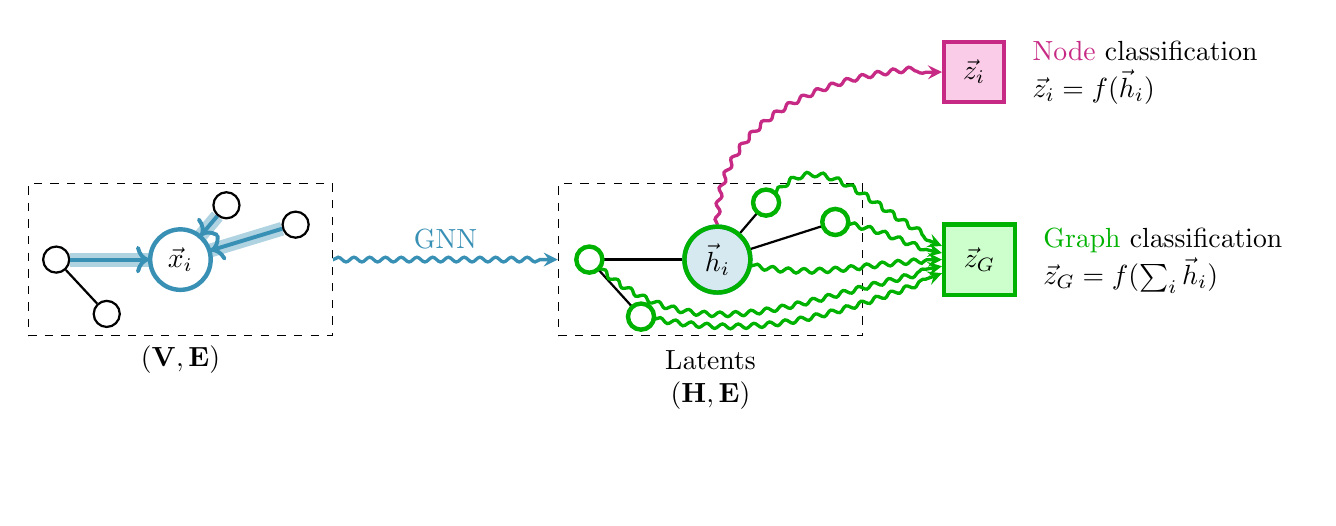
\begin{tikzpicture}[square/.style={regular polygon,regular polygon sides=4}]
        %% Graph 1 (V,E)
     	\node[circle, thick, draw] (0) {$\vec{x}_i$};
        \node[circle, thick, draw, above right=0.1em and 3em of 0] (1) {};
        \node[circle, thick, draw, above right=0.8em and 0.5em of 0] (2) {};
        \node[circle, thick, draw, left=of 0] (3) {};
        \node[circle, thick, draw, below left=0.8em and 1.5em of 0] (4) {};
        
        \draw[-, thick] (0) -- (1);
        \draw[-, thick] (0) -- (2);
        \draw[-, thick] (0) -- (3);
        \draw[-, thick] (4) -- (3);
        
        \node[rectangle, draw, dashed, minimum width=11em, minimum height=5.5em] (RR) {};
        \node[below=0em of RR] (l1) {$({\bf V}, {\bf E})$};

        %% Message passing
        \draw[->, line width=0.5mm, color=cyan!70!black] (1) -- (0);
        \draw[->, line width=0.5mm, color=cyan!70!black] (2) -- (0);
        \draw[->, line width=0.5mm, color=cyan!70!black] (3) -- (0);
        
        \path[draw,line width=5pt,-,cyan!70!black, opacity=0.4] (1) -- (0);
        \path[draw,line width=5pt,-,cyan!70!black, opacity=0.4] (2) -- (0);
        \path[draw,line width=5pt,-,cyan!70!black, opacity=0.4] (3) -- (0);
        
        \node[circle, ultra thick, draw, draw=cyan!70!black, text opacity=0] (m1) at ($(0)$) {$\vec{x}_i$};
    
    
        %% Graph 2 (H,E)
        \node[rectangle, draw, dashed, minimum width=11em, minimum height=5.5em, right=12.5em of 0] (AA) {};
        \node[below=0em of AA] (l1) {\begin{tabular}{c}
             Latents \\
             $({\bf H}, {\bf E})$
        \end{tabular}};
        
        \node[circle, ultra thick, draw, right=17em of 0, fill=cyan!70!black, draw=cyan!70!black,fill opacity=.2,text opacity=1] (0) {$\vec{h}_i$};
        \node[circle, thick, draw, above right=0.1em and 3em of 0] (1) {};
        \node[circle, thick, draw, above right= 0.8em and 0.5em of 0] (2) {};
        \node[circle, thick, draw, left=of 0] (3) {};
        \node[circle, thick, draw, below left=0.8em and 1.5em of 0] (4) {};
        
        \draw[-, thick] (0) -- (1);
        \draw[-, thick] (0) -- (2);
        \draw[-, thick] (0) -- (3);
        \draw[-, thick] (4) -- (3);
        
        %%%%%%%%%%%%%%%%%%%%%%%%%
        %% GNN connector
        \draw[-stealth, very thick, decoration={snake, pre length=0.01mm, segment length=2mm, amplitude=0.3mm, post length=1.5mm}, decorate,color=cyan!70!black] (RR) -- node[above] {GNN} (AA);
        %%%%%%%%%%%%%%%%%%%%%%%%%

        %% Node classification
        \node[square, ultra thick, draw, above right=of AA, fill=magenta, draw=magenta!80!black,fill opacity=.2,text opacity=1, draw opacity=1] (ZJ) {$\vec{z}_i$};
        \draw[-stealth, very thick, decoration={snake, pre length=0.01mm, segment length=2mm, amplitude=0.3mm, post length=1.5mm}, decorate,color=magenta!80!black] (0) to[out=90,in=180] (ZJ);
        \node[right=0em of ZJ] (zj1) {\begin{tabular}{l}
             \textcolor{magenta!80!black}{Node} classification \\
             $\vec{z}_i = f(\vec{h}_i)$
        \end{tabular}};
        \node[square, ultra thick, draw, right=of AA, fill=green, draw=green!70!black,fill opacity=.2,text opacity=1] (ZG) {$\vec{z}_G$};
        \node[right=0em of ZG] (zj1) {\begin{tabular}{l}
             \textcolor{green!70!black}{Graph} classification \\
             $\vec{z}_G = f(\sum_i \vec{h}_i)$
        \end{tabular}};
        \draw[-stealth, very thick, decoration={snake, pre length=0.01mm, segment length=2mm, amplitude=0.3mm, post length=1.5mm}, decorate,color=green!70!black] (0) to[out=350,in=180] (ZG);
        \draw[-stealth, very thick, decoration={snake, pre length=0.01mm, segment length=2mm, amplitude=0.3mm, post length=1.5mm}, decorate,color=green!70!black] (1) to[out=350,in=170] (ZG);
        \draw[-stealth, very thick, decoration={snake, pre length=0.01mm, segment length=2mm, amplitude=0.3mm, post length=1.5mm}, decorate,color=green!70!black] (2) to[out=45,in=160] (ZG);
        \draw[-stealth, very thick, decoration={snake, pre length=0.01mm, segment length=2mm, amplitude=0.3mm, post length=1.5mm}, decorate,color=green!70!black] (3) to[out=320,in=190] (ZG);
        \draw[-stealth, very thick, decoration={snake, pre length=0.01mm, segment length=2mm, amplitude=0.3mm, post length=1.5mm}, decorate,color=green!70!black] (4) to[out=350,in=200] (ZG);

        %%%%
        \node[circle, ultra thick, draw, draw=green!70!black, text opacity=0] (m1) at ($(0)$) {$\vec{h}_i$};
        
            \node[circle, ultra thick, draw, draw=green!70!black, text opacity=0] (m1) at ($(1)$) {};
        	    \node[circle, ultra thick, draw, draw=green!70!black, text opacity=0] (m1) at ($(2)$) {};
        	    \node[circle, ultra thick, draw, draw=green!70!black, text opacity=0] (m1) at ($(3)$) {};
        	    \node[circle, ultra thick, draw, draw=green!70!black, text opacity=0] (m1) at ($(4)$) {};

        \begin{lrbox}{0}
        \begin{scope}
            \node[square, ultra thick, draw, below right=of AA, fill=blue, draw=blue,fill opacity=.2,text opacity=1] (ZIJ) {$\vec{z}_{ij}$};
            \node[right=0em of ZIJ] (zj1) {\begin{tabular}{l}
                 \textcolor{blue}{Edge} classification \\
                 $\vec{z}_{ij} = f(\vec{h}_i,\vec{h}_j,\vec{e}_{ij})$
            \end{tabular}};
            \draw[-stealth, very thick, decoration={snake, pre length=0.01mm, segment length=2mm, amplitude=0.3mm, post length=1.5mm}, decorate,color=blue] (0) to[out=320,in=180] (ZIJ);
            \draw[-stealth, very thick, decoration={snake, pre length=0.01mm, segment length=2mm, amplitude=0.3mm, post length=1.5mm}, decorate,color=blue] (1) to[out=270,in=160] (ZIJ);

            %%%%
            \node[circle, ultra thick, draw, draw=blue, text opacity=0] (m1) at ($(0)$) {$\vec{h}_i$};
            	    
            \node[circle, ultra thick, draw, draw=blue, text opacity=0] (m1) at ($(1)$) {};
            	    
            \draw[<->, line width=0.5mm, color=blue] (1) -- (0);
            \path[draw,line width=5pt,-,blue, opacity=0.4] (1) -- (0);
        \end{scope}
        \end{lrbox}
    \end{tikzpicture}
        	
    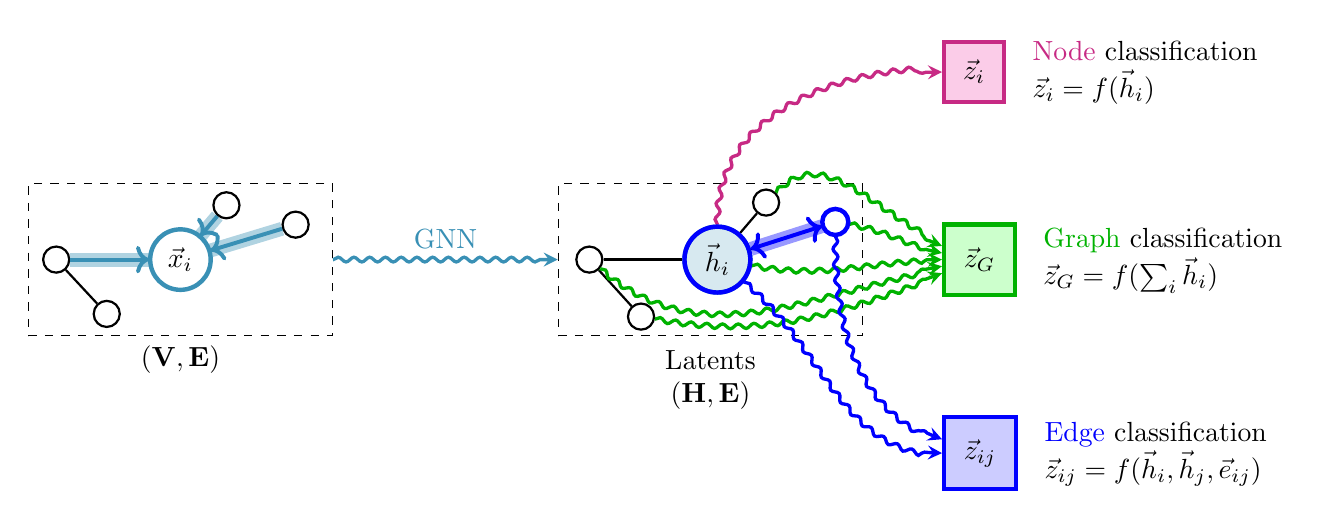
\begin{tikzpicture}[square/.style={regular polygon,regular polygon sides=4}]
        %% Graph 1 (V,E)
     	\node[circle, thick, draw] (0) {$\vec{x}_i$};
        \node[circle, thick, draw, above right=0.1em and 3em of 0] (1) {};
        \node[circle, thick, draw, above right=0.8em and 0.5em of 0] (2) {};
        \node[circle, thick, draw, left=of 0] (3) {};
        \node[circle, thick, draw, below left=0.8em and 1.5em of 0] (4) {};
        
        \draw[-, thick] (0) -- (1);
        \draw[-, thick] (0) -- (2);
        \draw[-, thick] (0) -- (3);
        \draw[-, thick] (4) -- (3);
        
        \node[rectangle, draw, dashed, minimum width=11em, minimum height=5.5em] (RR) {};
        \node[below=0em of RR] (l1) {$({\bf V}, {\bf E})$};

        %% Message passing
        \draw[->, line width=0.5mm, color=cyan!70!black] (1) -- (0);
        \draw[->, line width=0.5mm, color=cyan!70!black] (2) -- (0);
        \draw[->, line width=0.5mm, color=cyan!70!black] (3) -- (0);
        
        \path[draw,line width=5pt,-,cyan!70!black, opacity=0.4] (1) -- (0);
        \path[draw,line width=5pt,-,cyan!70!black, opacity=0.4] (2) -- (0);
        \path[draw,line width=5pt,-,cyan!70!black, opacity=0.4] (3) -- (0);
        
        \node[circle, ultra thick, draw, draw=cyan!70!black, text opacity=0] (m1) at ($(0)$) {$\vec{x}_i$};
    
    
        %% Graph 2 (H,E)
        \node[rectangle, draw, dashed, minimum width=11em, minimum height=5.5em, right=12.5em of 0] (AA) {};
        \node[below=0em of AA] (l1) {\begin{tabular}{c}
             Latents \\
             $({\bf H}, {\bf E})$
        \end{tabular}};
        
        \node[circle, ultra thick, draw, right=17em of 0, fill=cyan!70!black, draw=cyan!70!black,fill opacity=.2,text opacity=1] (0) {$\vec{h}_i$};
        \node[circle, thick, draw, above right=0.1em and 3em of 0] (1) {};
        \node[circle, thick, draw, above right= 0.8em and 0.5em of 0] (2) {};
        \node[circle, thick, draw, left=of 0] (3) {};
        \node[circle, thick, draw, below left=0.8em and 1.5em of 0] (4) {};
        
        \draw[-, thick] (0) -- (1);
        \draw[-, thick] (0) -- (2);
        \draw[-, thick] (0) -- (3);
        \draw[-, thick] (4) -- (3);
        
        %%%%%%%%%%%%%%%%%%%%%%%%%
        %% GNN connector
        \draw[-stealth, very thick, decoration={snake, pre length=0.01mm, segment length=2mm, amplitude=0.3mm, post length=1.5mm}, decorate,color=cyan!70!black] (RR) -- node[above] {GNN} (AA);
        %%%%%%%%%%%%%%%%%%%%%%%%%

        %% Node classification
        \node[square, ultra thick, draw, above right=of AA, fill=magenta, draw=magenta!80!black,fill opacity=.2,text opacity=1, draw opacity=1] (ZJ) {$\vec{z}_i$};
        \draw[-stealth, very thick, decoration={snake, pre length=0.01mm, segment length=2mm, amplitude=0.3mm, post length=1.5mm}, decorate,color=magenta!80!black] (0) to[out=90,in=180] (ZJ);
        \node[right=0em of ZJ] (zj1) {\begin{tabular}{l}
             \textcolor{magenta!80!black}{Node} classification \\
             $\vec{z}_i = f(\vec{h}_i)$
        \end{tabular}};
        \node[square, ultra thick, draw, right=of AA, fill=green, draw=green!70!black,fill opacity=.2,text opacity=1] (ZG) {$\vec{z}_G$};
        \node[right=0em of ZG] (zj1) {\begin{tabular}{l}
             \textcolor{green!70!black}{Graph} classification \\
             $\vec{z}_G = f(\sum_i \vec{h}_i)$
        \end{tabular}};
        \draw[-stealth, very thick, decoration={snake, pre length=0.01mm, segment length=2mm, amplitude=0.3mm, post length=1.5mm}, decorate,color=green!70!black] (0) to[out=350,in=180] (ZG);
        \draw[-stealth, very thick, decoration={snake, pre length=0.01mm, segment length=2mm, amplitude=0.3mm, post length=1.5mm}, decorate,color=green!70!black] (1) to[out=350,in=170] (ZG);
        \draw[-stealth, very thick, decoration={snake, pre length=0.01mm, segment length=2mm, amplitude=0.3mm, post length=1.5mm}, decorate,color=green!70!black] (2) to[out=45,in=160] (ZG);
        \draw[-stealth, very thick, decoration={snake, pre length=0.01mm, segment length=2mm, amplitude=0.3mm, post length=1.5mm}, decorate,color=green!70!black] (3) to[out=320,in=190] (ZG);
        \draw[-stealth, very thick, decoration={snake, pre length=0.01mm, segment length=2mm, amplitude=0.3mm, post length=1.5mm}, decorate,color=green!70!black] (4) to[out=350,in=200] (ZG);
        \node[square, ultra thick, draw, below right=of AA, fill=blue, draw=blue,fill opacity=.2,text opacity=1] (ZIJ) {$\vec{z}_{ij}$};
        \node[right=0em of ZIJ] (zj1) {\begin{tabular}{l}
             \textcolor{blue}{Edge} classification \\
             $\vec{z}_{ij} = f(\vec{h}_i,\vec{h}_j,\vec{e}_{ij})$
        \end{tabular}};
        \draw[-stealth, very thick, decoration={snake, pre length=0.01mm, segment length=2mm, amplitude=0.3mm, post length=1.5mm}, decorate,color=blue] (0) to[out=320,in=180] (ZIJ);
        \draw[-stealth, very thick, decoration={snake, pre length=0.01mm, segment length=2mm, amplitude=0.3mm, post length=1.5mm}, decorate,color=blue] (1) to[out=270,in=160] (ZIJ);

        %%%%
        \node[circle, ultra thick, draw, draw=blue, text opacity=0] (m1) at ($(0)$) {$\vec{h}_i$};
        	    
        \node[circle, ultra thick, draw, draw=blue, text opacity=0] (m1) at ($(1)$) {};
        	    
        \draw[<->, line width=0.5mm, color=blue] (1) -- (0);
        \path[draw,line width=5pt,-,blue, opacity=0.4] (1) -- (0);
    \end{tikzpicture}

\end{document}
